\section{Chess theorem}

\begin{theorem}[Von Neumann]
    In the game of chess, one and only one of the following alternatives holds:
\end{theorem}
\begin{enumerate}
    \item \textit{The White has a way to win, no matter what the Black does.}
    \item \textit{White has a strategy to guarantee a win, regardless of what Black does.}
    \item \textit{Both White and Black can force at least a draw, regardless of the opponent's actions.}
\end{enumerate}

\begin{proof}
    Assume the game has a finite length of $2K$ moves, where each player makes $K$ moves. 
    Let $a_i$ represent White's move at their $i$-th stage, and $b_i$ represent Black's corresponding move. 

    The first possibility in the theorem can be formulated as follows:
    \[\exists a_1 : \forall b_1 \exists a_2 : \forall b_2 \dots \exists a_K : \forall b_K \implies \text{white wins}\]
    Now, suppose this is false. 
    Then the negation is:
    \[\forall a_1 \exists b_1 : \forall a_2 : \exists b_2 : \dots \forall a_K : \exists b_K \implies \text{white does not win}\]
    This means Black has the possibility to prevent White from winning, ensuring at least a draw.
    
    If White does not have a winning strategy, then Black can secure at least a draw. 
    Similarly, if Black does not have a winning strategy, then White can secure at least a draw. 
    Therefore, if neither of the first two possibilities holds, the third one must be true.
\end{proof}

\subsection{Extension}
Von Neumann's theorem can be extended to any finite game of perfect information where the possible outcomes are either a win for one player or a tie. 
\begin{corollary}
    Consider a finite, perfect information game with two players, where the only possible outcomes are a win for one of the players or a tie. 
    Then, exactly one of the following holds:
\end{corollary}
\begin{enumerate}
    \item \textit{Player 1 has a winning strategy, no matter what the second player does.}
    \item \textit{Player 2 has a winning strategy, no matter what the second player does.}
\end{enumerate}
The possible solutions for a game are classified as follows:
\begin{itemize}
    \item \textit{Very weak solution}: the game has a rational outcome, but it is not accessible in practice, as with chess.
    \item \textit{Weak solution}: the outcome of the game is known, but the method to achieve it is not generally understood.
    \item \textit{Solution}: there exists an algorithm that can determine the outcome.
\end{itemize}
\begin{example}
    In the game of Chomp, players take turns removing tiles from a rectangular grid, where removing a tile also removes all tiles to its right and above. 
    The game ends when a player is unable to make a move, and the last player to play wins.

    In this scenario, we can distinguish between two types of solutions: a definite solution occurs when the grid is square, while a weak solution arises with a rectangular grid. 
    Let's consider a specific configuration, illustrated in the provided figure.
    \begin{figure}[H]
        \centering
        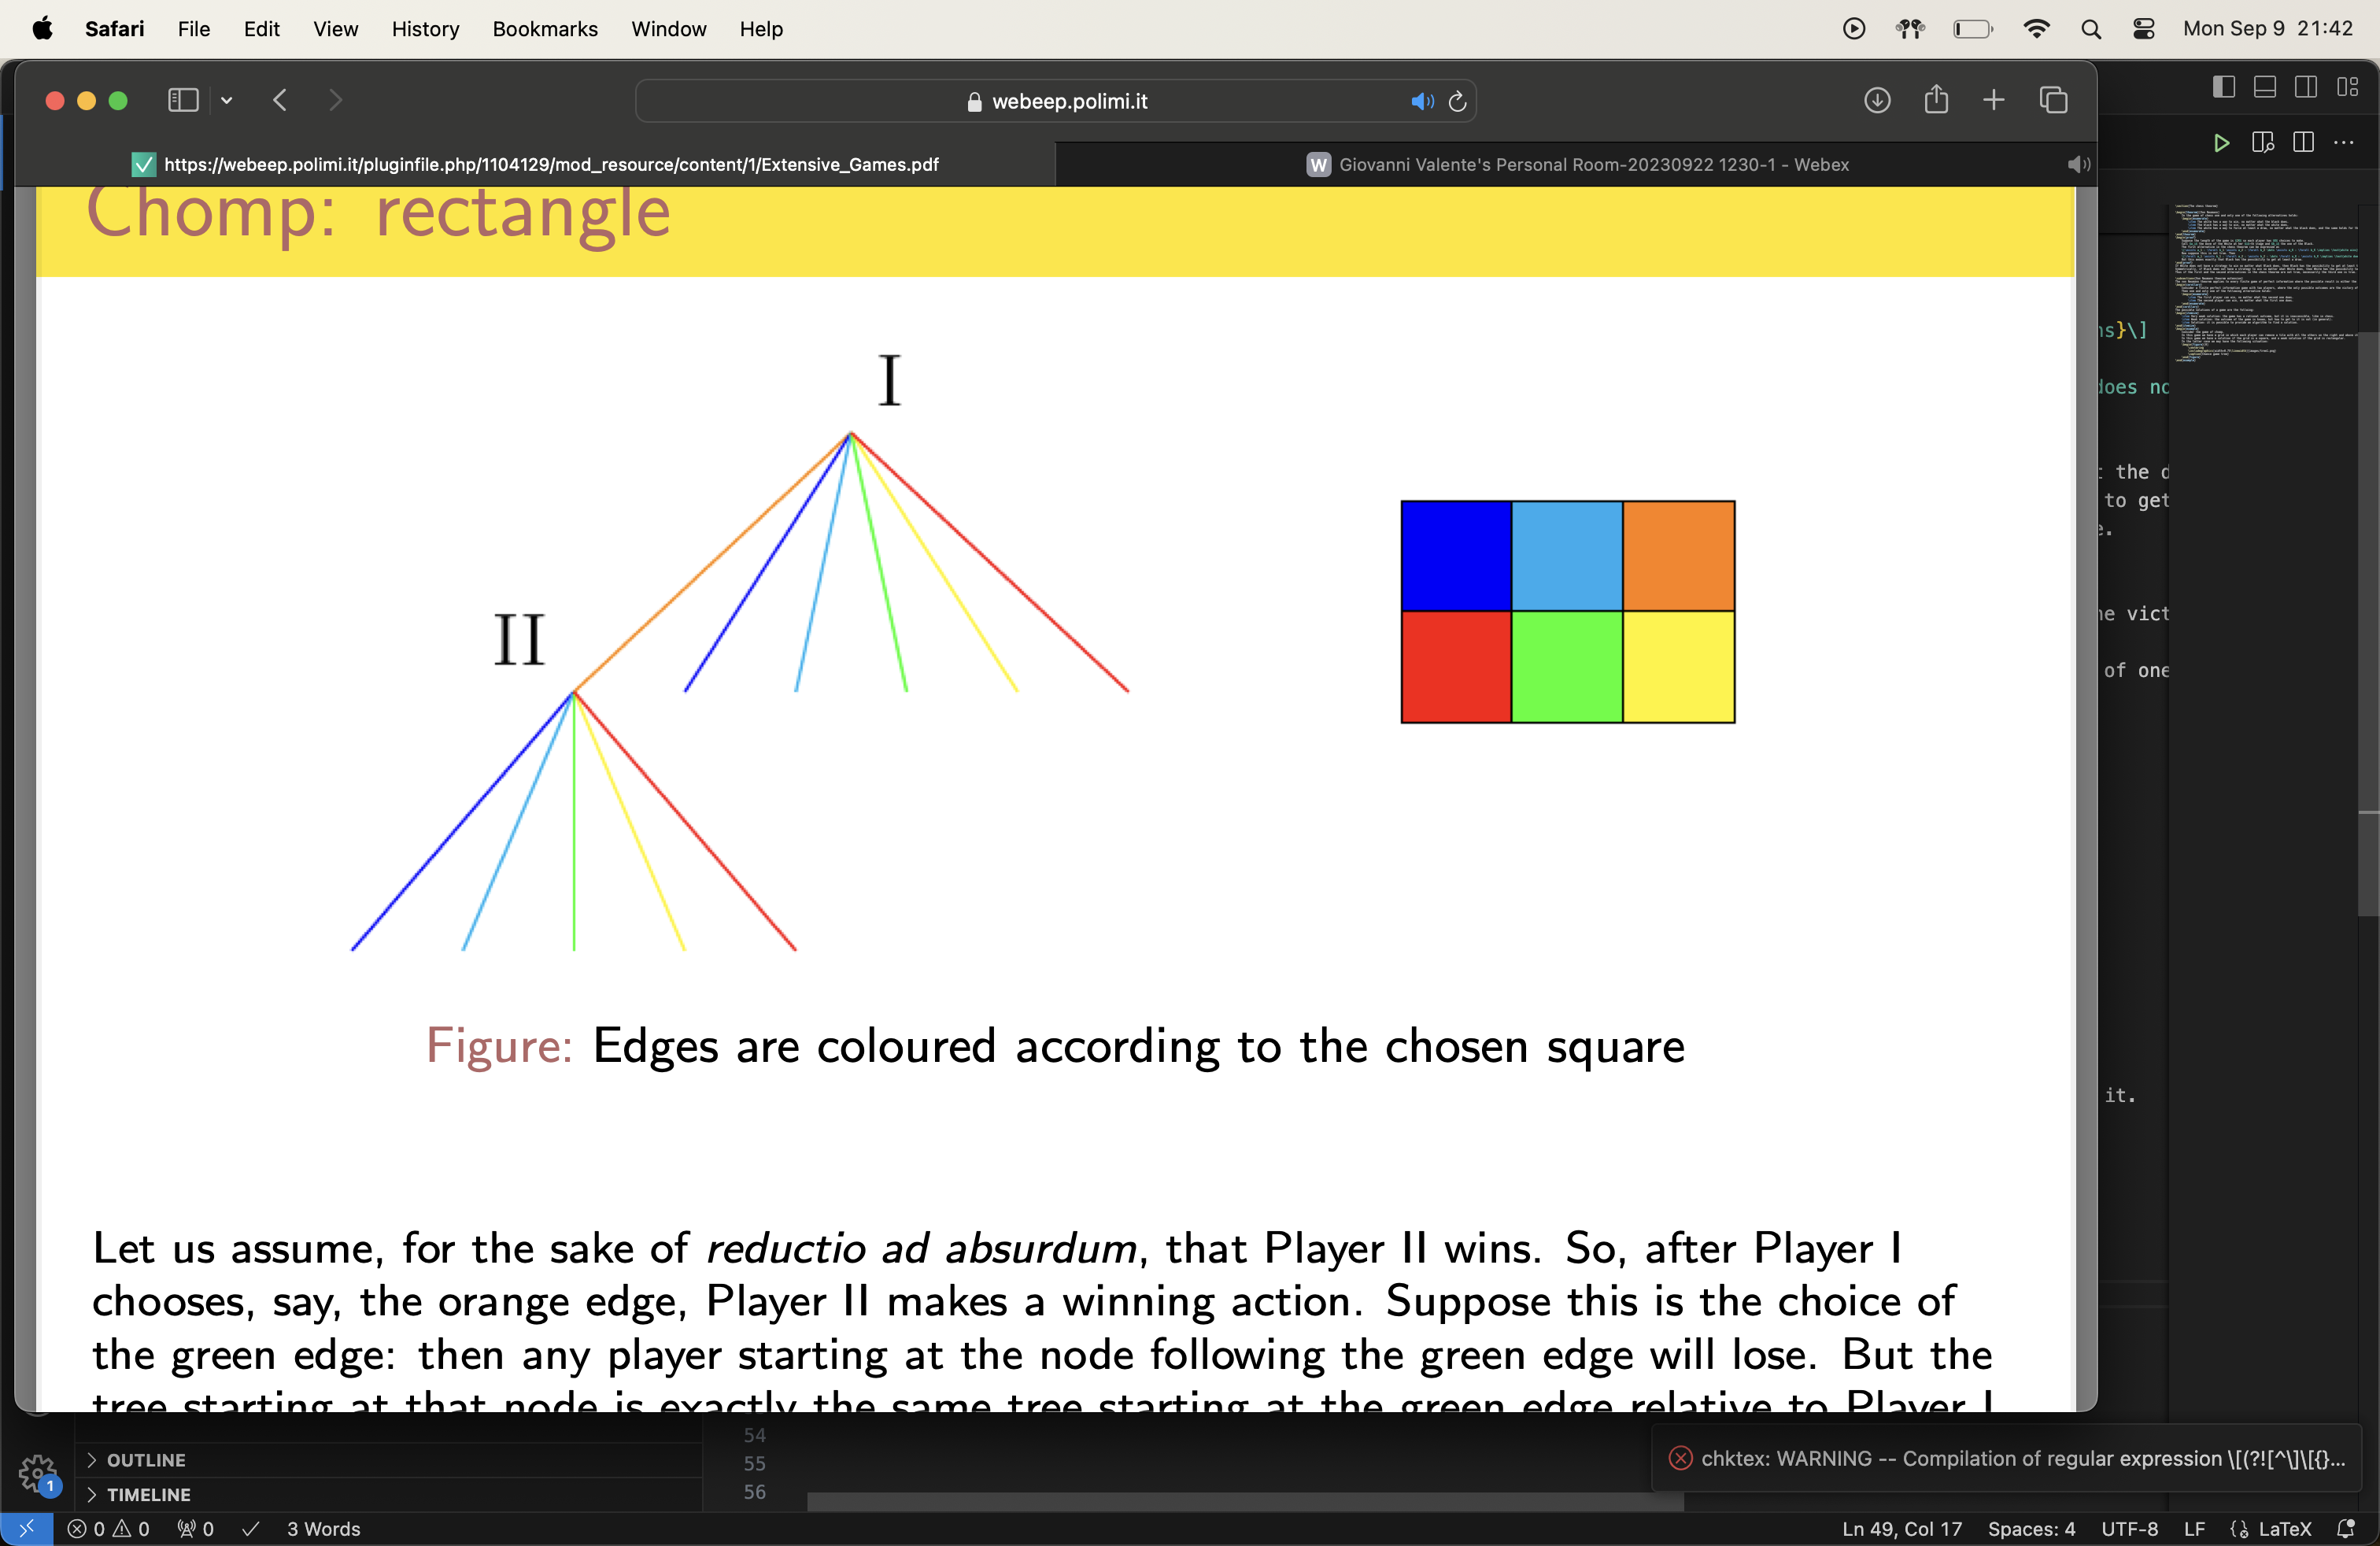
\includegraphics[width=0.75\linewidth]{images/chomp.png}
        \caption{Rectangular chomp}
    \end{figure}
    To explore the outcome of the game, let's assume for contradiction that Player 2 is the winner. 
    Suppose Player 1 chooses a particular edge (represented in orange), and then Player 2 makes a winning move by selecting another edge (the green edge). 
    If we examine the game state following this move, any player starting from the node that follows the green edge is destined to lose.

    However, this situation mirrors the tree of outcomes that begins at the green edge from Player 1's perspective. 
    This means that Player 1 has a move that guarantees a victory against Player 2's position. 
    Hence, the assumption that Player 2 can win leads to a contradiction, implying that Player 1 must be the one who wins the game.
    
    Thus, we conclude that Player 1 has a winning strategy in this instance of the game of Chomp.
\end{example}